\documentclass[a4paper,12pt]{report}

\usepackage[serbian, ngerman, english]{babel}
\usepackage[a4paper, inner=3cm, outer=3cm, top=2cm, bottom=2cm]{geometry}
\usepackage{blindtext}
\usepackage{microtype}
\usepackage{graphicx}
\usepackage{wrapfig}
\usepackage{enumitem}
\usepackage{fancyhdr}
\usepackage{amsmath}
\usepackage{index}
\usepackage[autostyle]{csquotes}
%\usepackage{booktabs}

\makeindex
%after this beguins the document

\begin{document}
\selectlanguage{serbian} 
%\renewcommand{\contentsname}{Sadržaj}
%\renewcommand{\chaptername}{Poglavlje}

\title{\Large{\textbf{Logistička i softmaks regresija (opis metoda, implementacija, primena nad podacima, komparativna analiza) i njihova primena kao aktivacione funkcije u neuronskim mrežama }}}
\author{Student: Danilo Veljović, broj indeksa: 1120}
\date{Novembar 6, 2020}
\maketitle
\let\cleardoublepage\clearpage
\tableofcontents

\pagenumbering{arabic}

\setcounter{page}{1}

\chapter{Uvod}
\ Termini poput veštačke inteligencije i mašinskog učenja su sve popularniji u savremenoj kulturi. Preko medija sve češće čujemo nagoveštaje vodećih naučnika iz ove oblasti da će sistemi koji koriste veštačku inteligenciju zameniti ljude na mnogim radnim mestima. Priča se da će prvo nestati najrepetitivniji poslovi poput vozača kamiona, radnika u skladištima, prodavaca i dr. Treba postaviti suštinsko pitanje zašto je to tako. Zašto će prvo rutinski poslovi nestati prvi? Odgovor na to pitanje daje prave smernice kada neko pokušava da shvati šta je to mašinsko učenje. \\ 

Mašinsko učenje vuče korene iz statistike. Slobodno rečeno, mašinsko učenje se može shvatiti kao primena statističkih metoda nad velikom količinom podataka, da bi se izvukle nekakve pravilnosti iz podataka. Te pravilnosti uočava model i opisuje ih različitim statističkim terminima. Model se može shvatiti kao parametrizovana funkcija koja može da \enquote{uči} iz podataka. Podaci se u mašinskom učenju dele na trening i test skupove. Trening skupovi imaju određene vrednosti za atribute i imaju izlaznu labelu klase kojoj pripadaju ili neke kontinualne vrednosti koju uzimaju. Model uzima jedan po jedan podatak iz trening skupa, ili čitavu grupu, i proba da napravi predikciju koje bi izlazne vrednosti mogle da odgovaraju tim ulazima. Kada vidi koliko njegova procena odudara od vrednosti labele za taj podatak, on se ispravi svoje parametre. Ovaj proces se naziva treniranje modela. Kada model optimizuje svoje parametre, i kada se odradi evaluacija modela, prelazi se na testiranje. Kada se model testira njemu se daju instance podataka koje nikad nije video. Za te instance on sada predviđa izlazne labele. \\

Posle ovog kratkog objašnjenja procesa mašinskog učenja, lako se može naslutiti odgovor na prethodno postavljeno pitanje o poslovima koje će prvo 
\enquote{progutati} inteligentni sistemi. Uzmimo primer radnika koji radi u skladištu i pomera kutije od mesta A do mesta B. Robot može da posmatra radnika koji nosi kutije i da zaključi da radnik na mestu A podigne kutiju, nosi je do mesta B i tu je spušta. To je njegov \enquote{trening skup} podataka. Kod ovakvog tipa inteligentih sistema najčešće se koriste konvolucione neuronske mreže za računarski vid, pomoću kojih sistem prima podatke o tome šta se dešava oko njega. Princip ostaje isti, sistem preko kamera, prima ulazne podatke, i ovo služi kao trening skup podataka. Trenira određen model, i kada se završi taj proces on može da izvede zadatak prenosa kutija. Ako se od sistema zahteva da radi nešto novo, slično prethodnom, on će probati to da uradi na jedan način, i u zavisnosti od ishoda \enquote{učiće} o tome gde je pogrešio, odnosno optimizovaće model. \\

%sad malo o konkretnim tehnikama, logističkoj, softmaks regresiji i pregled rada nadalje
Tehnike mašinskog učenja su srž inteligentnih sistema. Neki od važnijih modela mašinskog učenja su: 
\begin{itemize}
	\item \textit{Klasifikacija} predviđa klasu koja odgovara podatku
	\item \textit{Regresija} predviđa kontinualnu vrednost koja odgovara podatku
	\item \textit{Klasterizacija} je tehnika nenadgledanog učenja. Za razliku od tehnika nadgledanog učenja, o kojima je do sad bilo reči, kod nenadgledanog učenja nemamo informaciju o tome koji podatak ima kakvu klasu/vrednost. Zadatak klasterizacije je da one podatke koji su \enquote{slični} (mera sličnost se definiše kao parametar tehnike) grupiše zajedno.
	\item \textit{Neuronske mreže} su tehnika koja je donela revoluciju u svet mašinskog učenja i omogućila stvari poput računarskog vida i procesuiranja prirodnih jezika. Ideja za ovu tehniku dobijena je iz ideje ljudskog mozga. Cela neuronska mreža se sastoji iz veštačkih neurona, koji su međusobno povezani. Na slici 1.1 dat je prikaz jedne neuronske mreže. Neuronska mreža se sastoji iz tri sloja, \textit{ulaznog} sloja, mnoštvo \textit{skrivenih} slojeva i \textit{izlaznog sloja}. Ideja kod funkcionisanja neuronske mreže je da početni slojevi prepoznaju jako male delove sistema, npr kod računarskog vida prepoznaju ivice, kod procesuiranja prirodnih jezika prepoznaju pojedina slova. Skriveni slojevi prepoznaju složenije pojave, npr geometrijske figure ili tela, ili reči i rečenice. Na kraju izlazni neuroni se aktiviraju ako je prepoznato nešto. Primera radi, mreža može da se trenira da prepoznaje slike mačaka ili da prepoznaje da li je neka rečenica nosi pozitivna ili negativna osećanja. Ako mreža prepozna sliku mačke, ili ako je određena rečenica ima pozitivna osećanja, izlazni neuron se aktivira. 
\end{itemize}

\begin{figure}[ht]
	\centering
	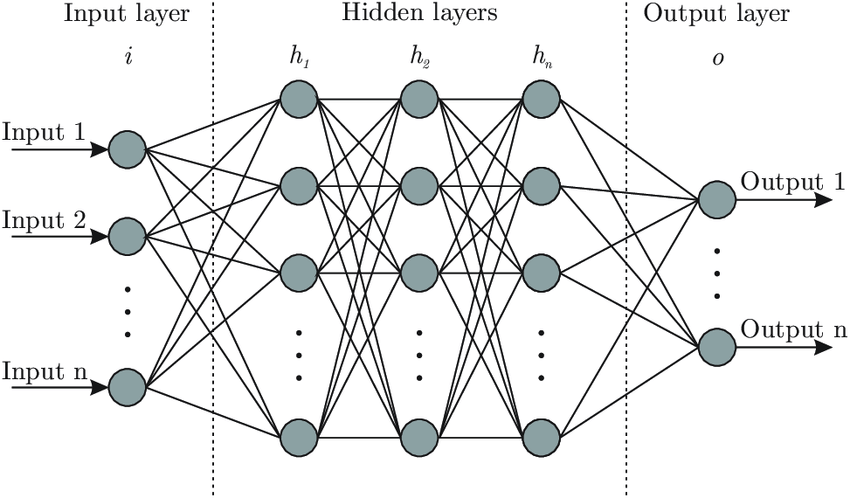
\includegraphics[width=8cm]{neuronske_mreze.png}
	\caption{Arhitektura neuronske mreže}\label{fig:prettypic}
\end{figure}

Jedna od tehnika koja se koristi za klasifikaciju se naziva \textit{logistička regresija}. Iako u nazivu sadrži reč \textit{regresija} ova tehnika se ne koristi za predviđanje kontinualne vrednosti, već za predviđanje da li neki podatak pripada nekoj klasi ili ne. U nastavku rada biće reči o matematičkim osnovama logističke regresije, o funkciji koja je vrlo slična logističkoj regresiji i vrlo često se koristi u sličnim situacijama - \textit{softmaks regresiji}. Implementiraćemo logističku i softmaks regresiju u programskom jeziku Python, primeniti je nad skupom podataka i evaluirati njihove performanse i napraviti komparativnu analizu obe tehnike. Na kraju rada biće dat prikaz primene logističke i softmaks regresije kao 
aktivacione funkcije (\enquote {\textit{threshold functions}}) kod neuronskih mreža.
\chapter{Teorijske osnove}

\section{Logistička regresija}

\section{Softmaks regresija}

\chapter{Implementacija}

\section{Logistička regresija}

\section{Softmaks regresija}

\chapter{Analiza rezultata}

\chapter{Primena kod neuronskih mreža}

\end{document}